\section{State machine}
    Le \textbf{Finite State Machine} (FSM) sono circuiti sequenziali che possono essere in uno stato tra un insieme finito di stati. 
    La transizione tra gli stati avviene in base a segnali di ingresso e può essere condizionata da segnali di clock e reset.

    \begin{minipage}[t]{1\columnwidth}
        \vspace{0pt} % <-- ensures top alignment
        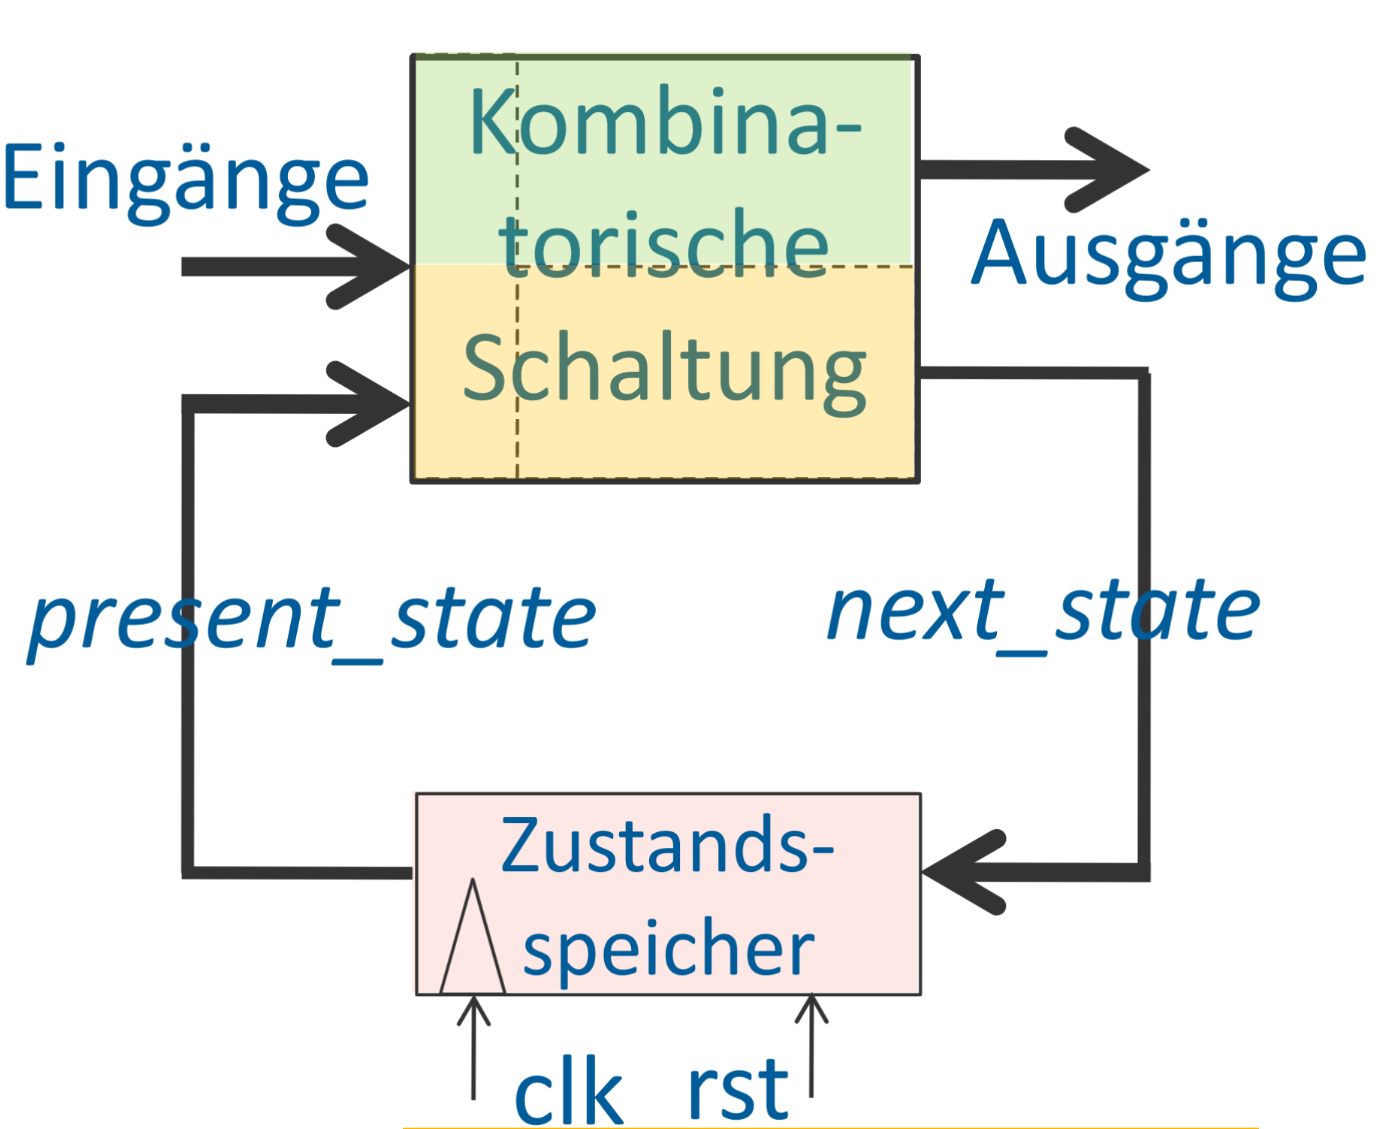
\includegraphics[width=\linewidth]{Images/FSMGeneralizzata.png}
    \end{minipage}%
    

% ==================================== CODICE SCHELETRO FSM ====================================
    \subsection{Codice scheletro FSM (f,g,z)}


% ==================================== CODIFICA DEGLI STATI ====================================
    \subsection{Codifica degli stati}
    Gli stati di una FSM possono essere codificati in diversi modi, tra cui:
    \begin{itemize}
        \item \textbf{Codifica binaria}: ogni stato è rappresentato da un codice binario unico.
        \item \textbf{Codifica Gray}: simile alla codifica binaria, ma le transizioni tra stati adiacenti cambiano solo un bit alla volta.
        \item \textbf{Codifica one-hot}: ogni stato è rappresentato da un bit attivo, con tutti gli altri bit a zero.
        \item \textbf{Codifica one-cold}: simile alla codifica one-hot, ma solo un bit è a zero e tutti gli altri sono attivi.
    \end{itemize}